\chapter{Fundamentos de imagens digitais}

Capítulo 2 de Gonzalez, \textit{Digital Image Processing}~\cite{gonzalez2006image}.

%%%%%%%%%%%%%%%%%%%%%%%%%%%%%%%%%%%%%%%%%%%%%%%%%%%%%%%%%%%%
\section{Elementos de percepção visual}

%%%%%%%%%%%%%%%%%%%%%%%%%%%%%%%%%%%%%%%%%%%%%%%%%%%%%%%%%%%%
\section{Luz e o espectro eletromagnético}

\begin{easylist}
& Frequência: $f$
& Comprimento de onda: $\lambda$
& Velocidade da luz: $ c = 3 \times 10^8 \text{m/s} \operatorname{m/s}$
& Constante de Planck: $ h = 6.6 \times 10^{-34} \text{Js (m$^2$kg/s)} $, $E = hf$.
\end{easylist}



\begin{figure}[!h]
  \begin{center}
    \begin{tabular}{c}
      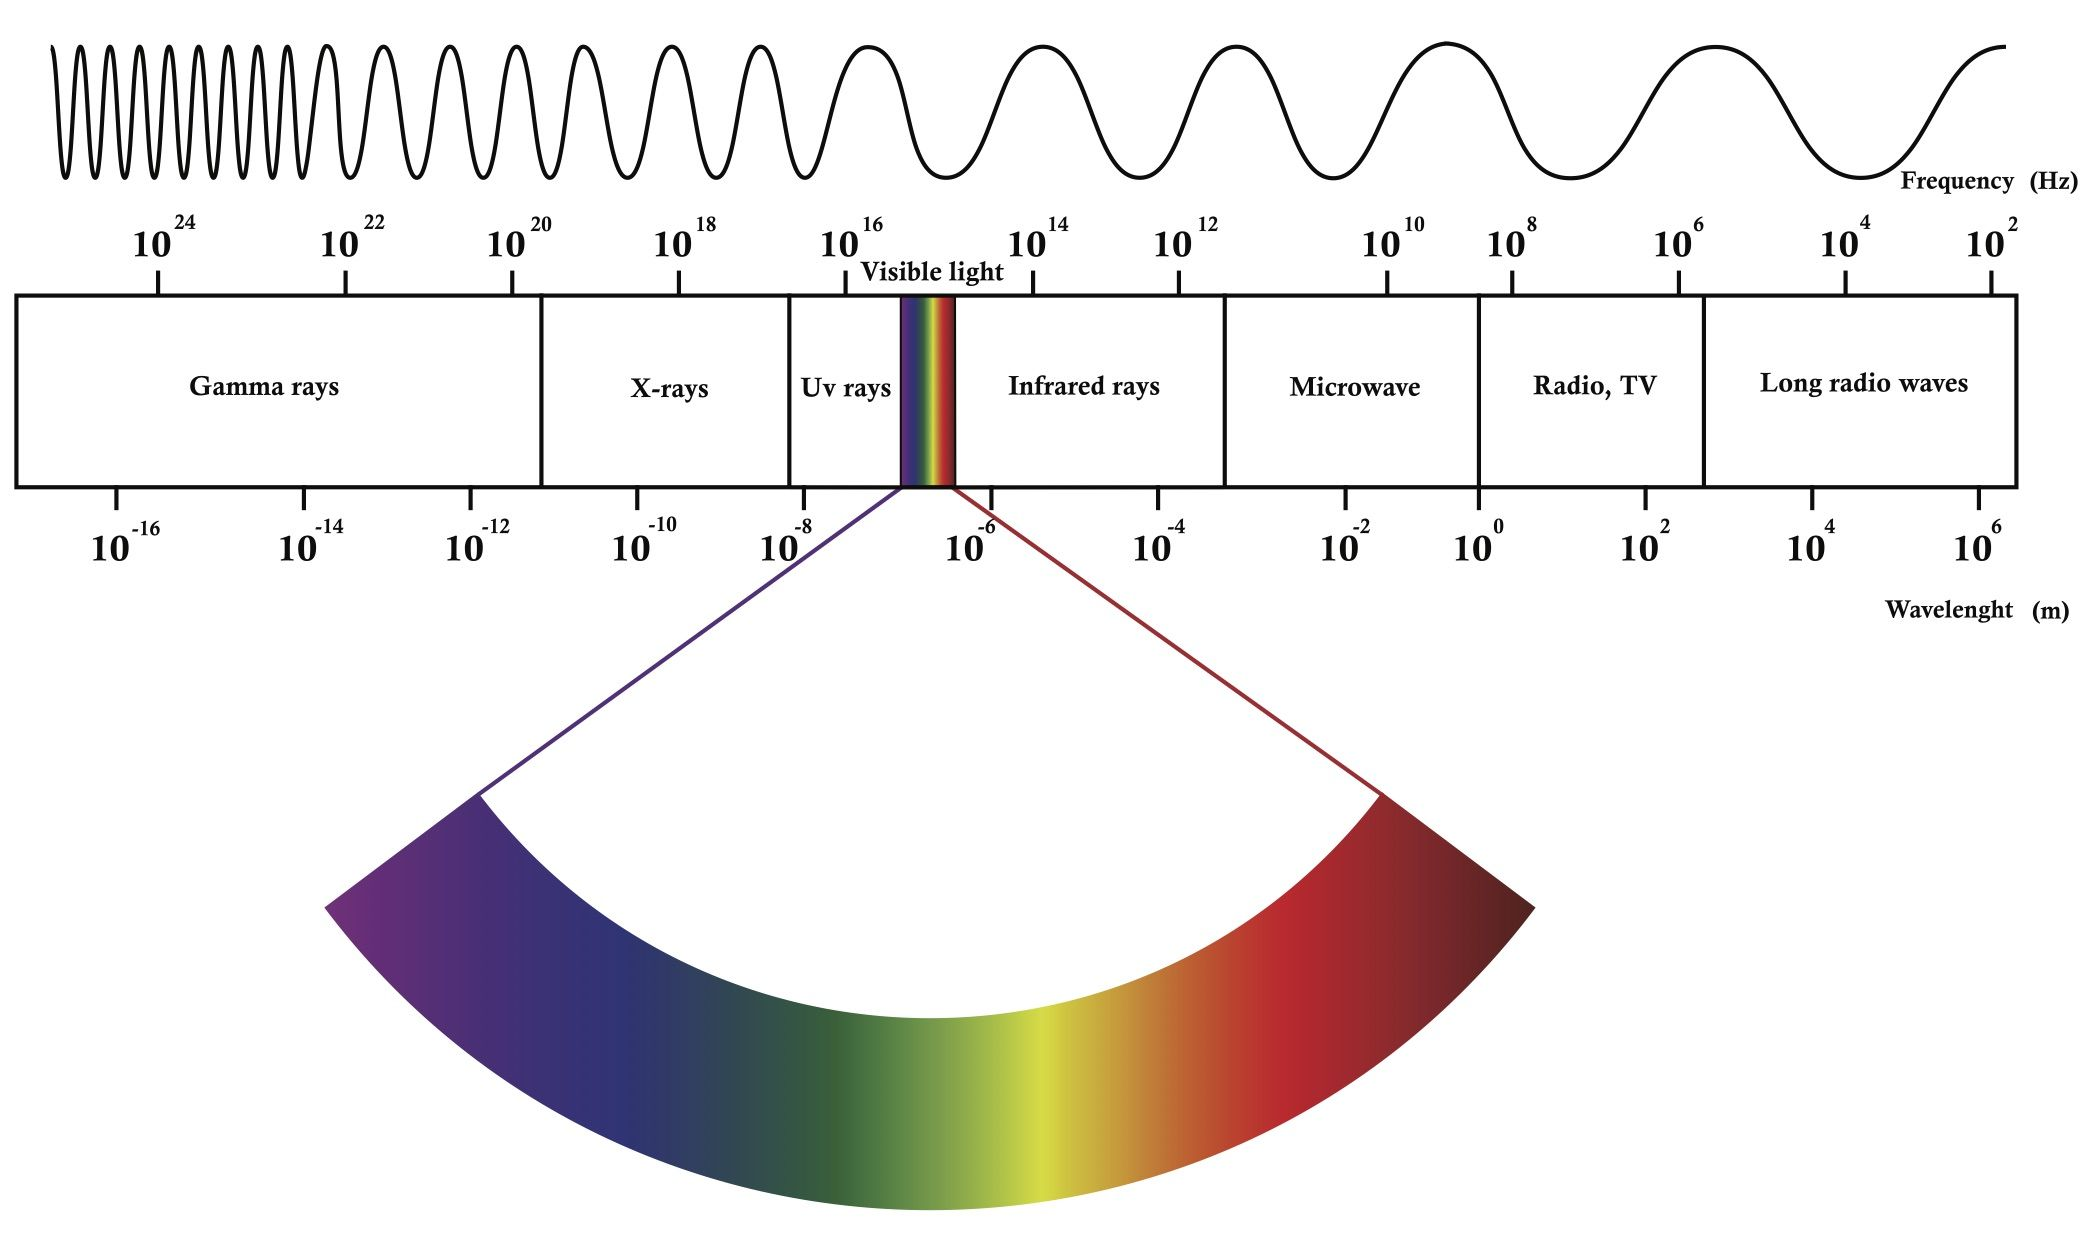
\includegraphics[width=0.7\textwidth]{images/02/spectrum.png}
    \end{tabular}
  \end{center}
  \caption{\label{fig:spectrum} Espectro eletromagnético}
\end{figure}


%%%%%%%%%%%%%%%%%%%%%%%%%%%%%%%%%%%%%%%%%%%%%%%%%%%%%%%%%%%%
\section{Aquisição de imagens}

\begin{easylist}
& Normalmente é feita através de componentes sensíveis a alguma faixa específica do espectro eletromagnético
&& Sensores simples: fotodiodo, fototransistor.
&& Sensores lineares: CCD linear.
&& Sensores em matriz: CCD de câmeras fotográficas, mouse ótico.
\end{easylist}

\begin{figure}[!h]
  \begin{center}
    \begin{tabular}{c}
      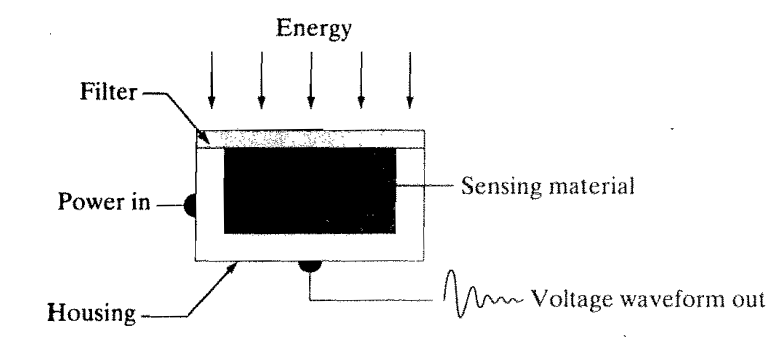
\includegraphics[width=0.8\textwidth]{images/02/sensor.png}
    \end{tabular}
  \end{center}
  \caption{\label{fig:sensor} Esquema de um sensor}
\end{figure}


%%%%%%%%%%%%%%%%%%%%%%%%%%%%%%%%%%%%%%%%%%%%%%%%%%%%%%%%%%%%
\section{Amostragem e quantização}

\begin{easylist}
& Amostragem: digitalização dos valores das coordenadas, tanto no espqço quanto no tempo.
& Quantização: digitalização dos valores das amplitudes
& Representação: 
&& Matriz
\end{easylist}

  \begin{equation*}
    f(i, j) =
    \begin{bmatrix}
      f(0, 0)   & f(0, 1)   & \dots  & f(0, N-1)   \\
      f(1, 0)   & f(1, 1)   & \dots  & f(1, N-1)   \\
      \vdots    & \vdots    & \ddots & \vdots      \\
      f(M-1, 0) & f(M-1, 1) & \dots  & f(M-1, N-1) 
    \end{bmatrix}      
  \end{equation*}
    
\begin{easylist}
&& Função
\end{easylist}
  
  \begin{align*}
    & f: \mathbb{Z}^2 \rightarrow \mathbb{Z} \\
    & f: \{0, \dots, M-1\} \times \{0, \dots, N-1\} \rightarrow \{0, \dots, L-1\}
  \end{align*}

\noindent
onde $L = 2^k$. $L$ é o intervalo dinâmico do sensor e $k$ é o número de bits necessário para representar $L$.

\vspace{1cm}
  
\begin{easylist}
&& Número de bits necessários para armazenar uma imagem $M \times N$:  
\end{easylist}

\[
  b = MNk  
\]

\begin{easylist}
&& Número de bytes necessários para armazenar uma imagem $M \times N$:  
\end{easylist}

\[
  B = MNk/8  
\]



\begin{easylist}
& Redimensionamento de imagem: \textit{zoom} ou \textit{resize}
&& \textit{Nearest neighbor}: ampliar uma imagem replicando cada pixel várias vezes.
&& Bilinear: ampliar uma imagem inserindo pixels calculados da interpolação linear entre os pixels mais próximos.
\end{easylist}

%%%%%%%%%%%%%%%%%%%%%%%%%%%%%%%%%%%%%%%%%%%%%%%%%%%%%%%%%%%%
\section{Relações entre pixels}

\begin{easylist}
& 4-adjacência: os vizinhos de $(x, y)$ são $(x, y-1)$, $(x, y+1)$, $(x-1, y)$ e $(x+1, y)$.
& D-adjacência: os vizinhos de $(x, y)$ são $(x-1, y-1)$, $(x-1, y+1)$, $(x+1, y+1)$ e $(x+1, y-1)$.
& 8-adjacência: os vizinhos de $(x, y)$ são a união da 4-adjacência e da D-adjacência.
\end{easylist}

\vspace{1cm}

\begin{table}[!h]
  \centering
  \begin{tabular}{|c|c|c|}
        \hline
        $(x-1, y-1)$ & $(x, y-1)$ & $(x+1, y-1)$ \\
        \hline
        $(x-1, y  )$ & $(x, y  )$ & $(x+1, y  )$ \\
        \hline
        $(x-1, y+1)$ & $(x, y+1)$ & $(x+1, y+1)$ \\
        \hline
  \end{tabular}
  \caption{Disposição dos pixels na vizinhança de $(x, y)$.}
\end{table}


\begin{easylist}
& Distância: é uma relação entre dois pixels $p$ e $q$ com as propriedades listadas abaixo.  
\end{easylist}

  \begin{align*}
    & 1.\; D(p, q) \geq 0 \\
    & 2.\; D(p, q) = 0 \Leftrightarrow p = q \\
    & 3.\; D(p, q) = D(q, p)                 && \text{simetria} \\
    & 4.\; D(p, q) \leq D(p, z) + D(z, q)    && \text{desigualdade triangular}    \\
  \end{align*}

\begin{easylist}
&& Distância Euclidiana:           $D_e(p, q) = \sqrt{(p_x - q_x)^2 + (p_y - q_y)^2}$
&& Distância \textit{city-block}:  $D_4(p, q) = |p_x - q_x| + |p_y - q_y|$
&& Distância \textit{chessboard}:  $D_8(p, q) = \max(|p_x - q_x|, |p_y - q_y|)$
\end{easylist}


%%%%%%%%%%%%%%%%%%%%%%%%%%%%%%%%%%%%%%%%%%%%%%%%%%%%%%%%%%%%
\section{Ferramentas matemáticas}

\begin{easylist}
& Operações lineares: seja $H$ uma operação cuja entrada e saída são imagens, sejam $f$ e $g$ duas imagens, e $a$ e $b$, dois escalares. A operação $H$ é dita linear se segue a relação abaixo

  \[
    H(af + bg) = aH(f) + bH(g)
  \]

& Operações não-lineares: uma operação é dita não-linear se não é linear.
\end{easylist}

